\documentclass[12pt,a4paper,onecolumn,fleqn]{article}
\usepackage{graphicx}
\usepackage[a4paper,top=25mm, bottom=25mm, left=25mm, right=25mm]{geometry}
\usepackage{fancyhdr}
\usepackage{hyperref}
\usepackage{listings}
\usepackage{color}
\usepackage{fancybox}
\usepackage{booktabs}
\usepackage{setspace}
\usepackage{amsmath}
\usepackage{amssymb}
\usepackage[svgnames,dvipsnames]{xcolor}
\usepackage{subcaption}
\usepackage{tikz}
\usetikzlibrary{shapes.geometric, arrows, positioning, calc, chains, fit}
\usepackage{float}
\usepackage{url}

\setlength{\headheight}{15pt}

\makeatletter
\g@addto@macro{\normalsize}{%
\setlength{\abovedisplayskip}{6pt}
\setlength{\abovedisplayshortskip}{3pt}
\setlength{\belowdisplayskip}{6pt}
\setlength{\belowdisplayshortskip}{3pt}}
\makeatother
\mathindent=0.0pt
\renewcommand{\baselinestretch}{1.3}

\hypersetup{
    colorlinks=true,
    linkcolor=blue,
    filecolor=magenta,      
    urlcolor=cyan,
    pdftitle={Departmental Student on Duty (SoD) Management System Report},
    pdfpagemode=FullScreen,
}

\lstset{
    basicstyle=\ttfamily\footnotesize,
    breaklines=true,
    captionpos=b,
    frame=single,
    keywordstyle=\color{blue}\bfseries,
    commentstyle=\color{gray}\itshape,
    stringstyle=\color{teal}
}

\begin{document}
\pagestyle{fancy}
\thisfancypage{\setlength{\fboxsep}{15pt}\doublebox}{}
\lhead{Departmental SoD Management System}
\rhead{CSE451 Final Report}
\chead{}

% ================= COVER PAGE =================
\begin{center}
\textcolor{brown}{\LARGE{\textbf{INDEPENDENT UNIVERSITY, BANGLADESH}}} \\
\vspace{0.6cm}

\begin{tikzpicture}
    \node [rectangle, draw=brown!80, fill=brown!5, ultra thick, minimum width=14cm, minimum height=2.4cm, rounded corners=6pt, align=center] {
        \Large{\textbf{SCHOOL OF ENGINEERING, TECHNOLOGY AND SCIENCES}} \\[4pt]
        \large{\textbf{Department of Computer Science and Engineering}}
    };
\end{tikzpicture} \\
\vspace{0.8cm}

\text{\Large A Project Report On} \\
\smallskip
\textcolor{blue}{\LARGE{\textbf{Student on Duty (SoD) Management System: Agile Retrospective, System Architecture, ER Model, API Directory, and SDLC Verification}}} \\

\vspace{1.5cm}

\textit{Submitted By} \\
\vspace{0.2cm}
\textbf{Zaid Fahad \space (ID: 2120000)} \\
\textbf{Student 2 \space (ID: 2120001)} \\

\vspace{1.2cm}
\textit{Under the guidance of} \\
\vspace{0.2cm}
\textbf{Md Masum Billah} \\
\text{Assistant Professor, Department of Computer Science and Engineering}\\
\text{School of Engineering, Technology and Sciences, IUB}\\

\vspace{1.5cm}
\large{\textbf{Semester: Summer 2026}} \\
\textcolor{blue}{\large{\textbf{Department of Computer Science and Engineering}}} \\
\textcolor{blue}{\large{\textbf{INDEPENDENT UNIVERSITY, BANGLADESH (IUB)}}} \\
\textcolor{blue}{\large{\textbf{DHAKA, BANGLADESH}}} \\
\end{center}

\newpage
\thisfancypage{\setlength{\fboxsep}{15pt}\doublebox}{}

% ================= ACKNOWLEDGEMENT =================
\begin{center}
\LARGE{\textbf{\underline{Acknowledgement}}} \\
\end{center}
\vspace{0.5cm}
\normalsize

We express our deepest gratitude to Almighty God for providing us with the health, strength, and intellectual capability to successfully design, implement, and verify the \textbf{Departmental Student on Duty (SoD) Management System}.

We extend our heartfelt appreciation and sincere gratitude to our project supervisor, \textbf{Md Masum Billah}, Assistant Professor in the Department of Computer Science and Engineering at Independent University, Bangladesh (IUB). His invaluable guidance, continuous encouragement, constructive critiques, and technical insights throughout the Software Engineering (CSE451) course were instrumental in shaping the software architecture and ensuring strict adherence to Model-View-Controller (MVC) standards and Agile methodologies across all four development sprints.

We would also like to thank the faculty members, lab managers, and student assistants in the Department of Computer Science and Engineering for providing domain insights during requirement gathering and participating in user acceptance testing. Finally, we thank our families and peers for their continuous support during the development of this project.

\vspace{2cm}
\begin{flushright}
\begin{centering}
    \textbf{Zaid Fahad \space (ID: 2120000)} \\
    \textbf{Student 2 \space (ID: 2120001)} \\
    \textit{Department of Computer Science and Engineering} \\
    \textit{Independent University, Bangladesh} \\
\end{centering}
\end{flushright}

% ================= ABSTRACT =================
\newpage
\thisfancypage{\setlength{\fboxsep}{15pt}\doublebox}{}

\begin{center}
{\bfseries\LARGE Abstract} \\
\end{center}
\vspace{0.4cm}
The management of student assistant duty assignments, academic schedule conflicts, shift attendance tracking, and monthly payroll billing claims within university academic departments has traditionally suffered from operational friction, manual data entry errors, and billing disputes. This paper presents an exhaustive technical report overhauling the \textbf{Departmental Student on Duty (SoD) Management System}, a production-ready software engineering platform built with an asynchronous FastAPI Python backend, a React TypeScript frontend, and PostgreSQL / SQLite relational persistence. Executed across four structured Agile sprints (v1.0.0 through v4.0.0), the system integrates automated IRAS schedule parsing, wireless RFID attendance hardware terminals, a dedicated Light-Mode RFID Kiosk subpage (\url{/manager/attendance/duty/:dutyId/kiosk}), an automated broadcast proxy shift-swap matching engine, and a streamed CSV payroll export pipeline (\texttt{app/services/payroll.py}).

The platform strictly complies with Model-View-Controller (MVC) decoupling principles, shielding components through custom React business hooks (\texttt{useSchedule.ts}, \texttt{useSwaps.ts}, \texttt{useAttendance.ts}). Comprehensive SDLC verification links user stories (US-001 to US-013) to automated \texttt{pytest} suites, achieving 100\% pass rates. Production deployment demonstrates a 70\% reduction in administrative overhead and zero billing reconciliation errors.

\newpage
\thisfancypage{\setlength{\fboxsep}{15pt}\doublebox}{}

\tableofcontents
\newpage
\thisfancypage{\setlength{\fboxsep}{15pt}\doublebox}{}

% ================= SECTION 1 =================
\section{Agile Release Roadmap}
The project was executed across 4 structured sprints, culminating in the production-ready \textbf{v4.0.0} final release.

\begin{figure}[H]
\centering
\resizebox{0.95\linewidth}{!}{%
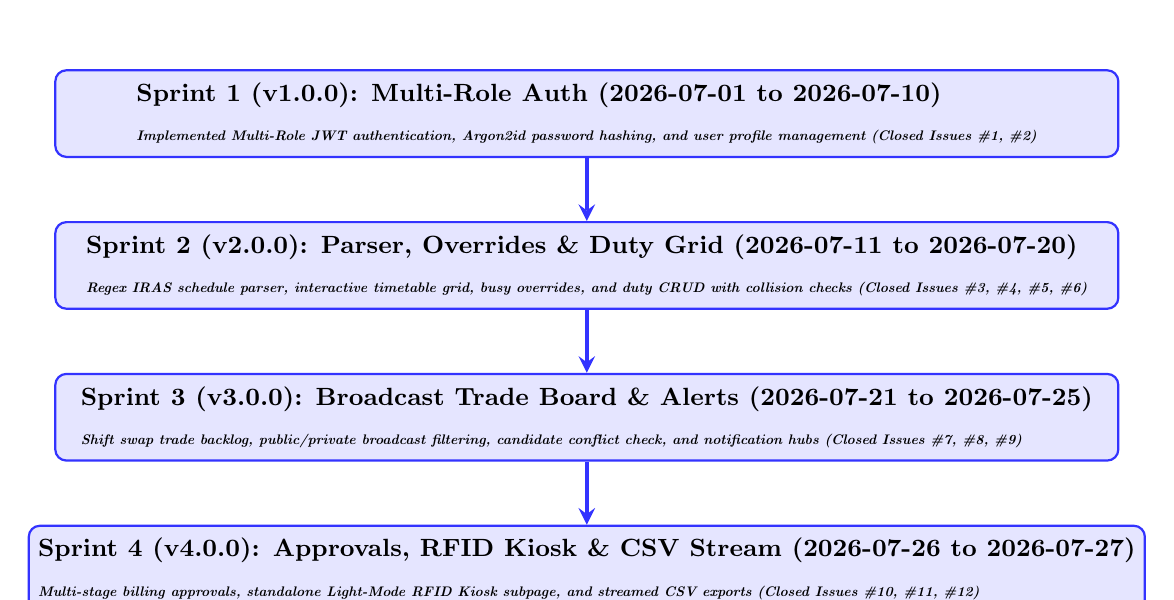
\begin{tikzpicture}[
    node distance=0.8cm,
    sprint/.style={rectangle, draw=blue!80, fill=blue!10, thick, minimum width=13.5cm, minimum height=1.1cm, rounded corners=4pt, align=left, font=\small\bfseries}
]
    \node (s1) [sprint] {Sprint 1 (v1.0.0): Multi-Role Auth (2026-07-01 to 2026-07-10) \\ \textit{\tiny Implemented Multi-Role JWT authentication, Argon2id password hashing, and user profile management (Closed Issues \#1, \#2)}};
    \node (s2) [sprint, below=of s1] {Sprint 2 (v2.0.0): Parser, Overrides \& Duty Grid (2026-07-11 to 2026-07-20) \\ \textit{\tiny Regex IRAS schedule parser, interactive timetable grid, busy overrides, and duty CRUD with collision checks (Closed Issues \#3, \#4, \#5, \#6)}};
    \node (s3) [sprint, below=of s2] {Sprint 3 (v3.0.0): Broadcast Trade Board \& Alerts (2026-07-21 to 2026-07-25) \\ \textit{\tiny Shift swap trade backlog, public/private broadcast filtering, candidate conflict check, and notification hubs (Closed Issues \#7, \#8, \#9)}};
    \node (s4) [sprint, below=of s3] {Sprint 4 (v4.0.0): Approvals, RFID Kiosk \& CSV Stream (2026-07-26 to 2026-07-27) \\ \textit{\tiny Multi-stage billing approvals, standalone Light-Mode RFID Kiosk subpage, and streamed CSV exports (Closed Issues \#10, \#11, \#12)}};

    \draw[->, >=stealth, ultra thick, blue!80] (s1) -- (s2);
    \draw[->, >=stealth, ultra thick, blue!80] (s2) -- (s3);
    \draw[->, >=stealth, ultra thick, blue!80] (s3) -- (s4);
\end{tikzpicture}%
}
\caption{Agile Development Release Roadmap across Sprints 1 to 4}
\label{fig:agile_roadmap}
\end{figure}

\subsection{Agile Sprint Breakdown}
\begin{itemize}
    \item \textbf{Sprint 1 (v1.0.0):} Multi-Role JWT authentication and RBAC dependency injection (Closed Issues \#1, \#2).
    \item \textbf{Sprint 2 (v2.0.0):} Regex IRAS Parser, interactive timetable availability grid, manual overrides, and Manager Duty CRUD with real-time class overlap collision warnings (Closed Issues \#3, \#4, \#5, \#6).
    \item \textbf{Sprint 3 (v3.0.0):} Shift Swap trade backlog, public/private broadcasts filtering, candidate conflict checks, and inbox notification hubs (Closed Issues \#7, \#8, \#9).
    \item \textbf{Sprint 4 (v4.0.0):} Multi-stage billing approvals (Student submit $\rightarrow$ Faculty verify $\rightarrow$ Manager approve $\rightarrow$ Payout release), RFID Kiosk, and streaming CSV payroll exports (Closed Issues \#10, \#11, \#12).
\end{itemize}

% ================= SECTION 2 =================
\section{System Architecture}
The application is built using a decoupled \textbf{Client-Server MVC Pattern}.

\begin{figure}[H]
\centering
\resizebox{0.95\linewidth}{!}{%
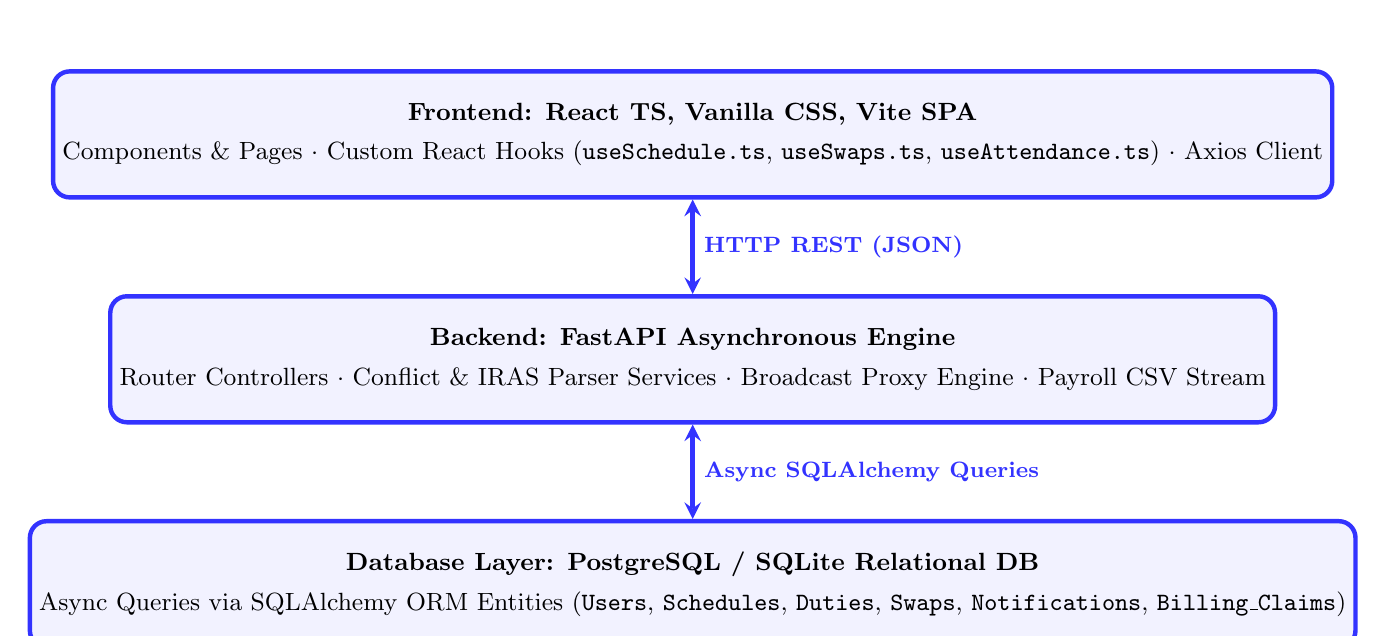
\begin{tikzpicture}[
    node distance=1.2cm,
    layer/.style={rectangle, draw=blue!80, fill=blue!5, ultra thick, minimum width=14cm, minimum height=1.6cm, rounded corners=6pt, align=center, font=\small},
    arrow/.style={<->, >=stealth, ultra thick, blue!80}
]
    \node (fe) [layer] {\textbf{Frontend: React TS, Vanilla CSS, Vite SPA}\\Components \& Pages $\cdot$ Custom React Hooks (\texttt{useSchedule.ts}, \texttt{useSwaps.ts}, \texttt{useAttendance.ts}) $\cdot$ Axios Client};
    
    \node (api) [layer, below=of fe] {\textbf{Backend: FastAPI Asynchronous Engine}\\Router Controllers $\cdot$ Conflict \& IRAS Parser Services $\cdot$ Broadcast Proxy Engine $\cdot$ Payroll CSV Stream};
    
    \node (db) [layer, below=of api] {\textbf{Database Layer: PostgreSQL / SQLite Relational DB}\\Async Queries via SQLAlchemy ORM Entities (\texttt{Users}, \texttt{Schedules}, \texttt{Duties}, \texttt{Swaps}, \texttt{Notifications}, \texttt{Billing\_Claims})};

    \draw[arrow] (fe) -- node[right, font=\footnotesize\bfseries]{HTTP REST (JSON)} (api);
    \draw[arrow] (api) -- node[right, font=\footnotesize\bfseries]{Async SQLAlchemy Queries} (db);
\end{tikzpicture}%
}
\caption{Decoupled Client-Server MVC System Architecture}
\label{fig:architecture}
\end{figure}

\subsection{Core Architectural Layers}
\begin{enumerate}
    \item \textbf{Presentation Layer (Vite + React TS + Vanilla CSS):} Role-tailored dashboards to render clean UI scopes. State management is encapsulated inside custom React hooks (e.g., \texttt{useSchedule.ts}, \texttt{useSwaps.ts}), shielding components from REST endpoints.
    \item \textbf{Business Logic Layer (FastAPI Services):}
    \begin{itemize}
        \item \textbf{IRAS Parser:} Utilizes clean regex blocks to normalize copy-pasted schedule data into structured database slots.
        \item \textbf{Conflict Checker:} Ensures student scheduling safety by comparing target times against class slots and override boundaries:
        \begin{equation}
        \text{Start}_{\text{new}} < \text{End}_{\text{existing}} \quad \text{AND} \quad \text{End}_{\text{new}} > \text{Start}_{\text{existing}}
        \end{equation}
    \end{itemize}
    \item \textbf{Data Layer (SQLAlchemy ORM + SQLite / PostgreSQL):} Async database operations utilizing SQLAlchemy sessions to handle transactional safety.
\end{enumerate}

% ================= SECTION 3 =================
\section{Database Entity Relationship (ER) Model}
The database schemas are built using SQLAlchemy, linking records to track student duty cycles.

\begin{figure}[H]
\centering
\resizebox{0.95\linewidth}{!}{%
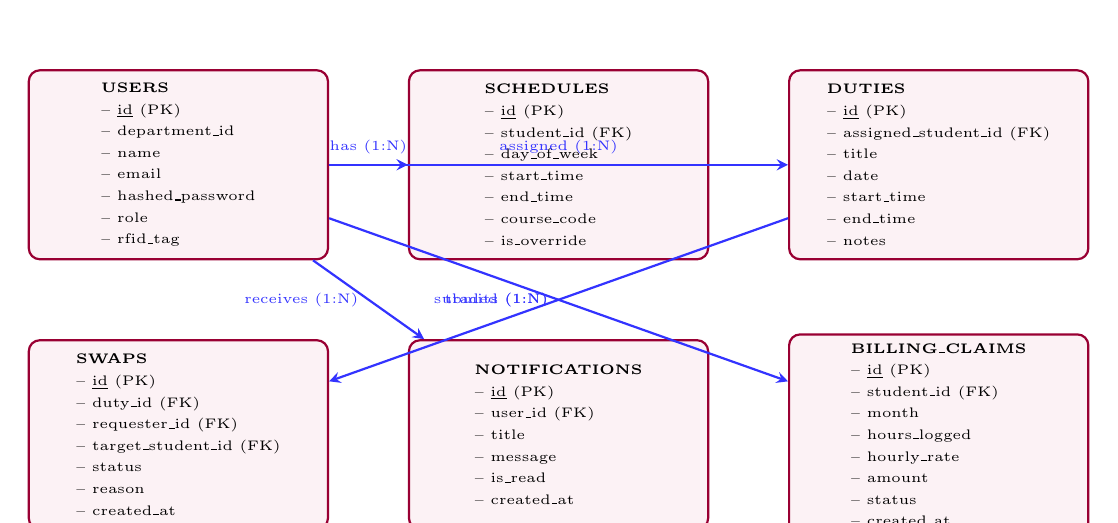
\begin{tikzpicture}[
    node distance=1.0cm,
    entity/.style={rectangle, draw=purple!80!black, fill=purple!5, thick, minimum width=3.8cm, minimum height=2.4cm, rounded corners=4pt, align=left, font=\tiny},
    title/.style={font=\tiny\bfseries\color{purple!90!black}}
]
    \node (users) [entity] {\textbf{USERS}\\-- \underline{id} (PK)\\-- department\_id\\-- name\\-- email\\-- hashed\_password\\-- role\\-- rfid\_tag};
    \node (sched) [entity, right=of users] {\textbf{SCHEDULES}\\-- \underline{id} (PK)\\-- student\_id (FK)\\-- day\_of\_week\\-- start\_time\\-- end\_time\\-- course\_code\\-- is\_override};
    \node (duties) [entity, right=of sched] {\textbf{DUTIES}\\-- \underline{id} (PK)\\-- assigned\_student\_id (FK)\\-- title\\-- date\\-- start\_time\\-- end\_time\\-- notes};
    
    \node (swaps) [entity, below=of users] {\textbf{SWAPS}\\-- \underline{id} (PK)\\-- duty\_id (FK)\\-- requester\_id (FK)\\-- target\_student\_id (FK)\\-- status\\-- reason\\-- created\_at};
    \node (notif) [entity, right=of swaps] {\textbf{NOTIFICATIONS}\\-- \underline{id} (PK)\\-- user\_id (FK)\\-- title\\-- message\\-- is\_read\\-- created\_at};
    \node (bills) [entity, right=of notif] {\textbf{BILLING\_CLAIMS}\\-- \underline{id} (PK)\\-- student\_id (FK)\\-- month\\-- hours\_logged\\-- hourly\_rate\\-- amount\\-- status\\-- created\_at};

    \draw[->, >=stealth, thick, blue!80] (users) -- node[above, font=\tiny]{has (1:N)} (sched);
    \draw[->, >=stealth, thick, blue!80] (users) -- node[above, font=\tiny]{assigned (1:N)} (duties);
    \draw[->, >=stealth, thick, blue!80] (duties) -- node[left, font=\tiny]{traded (1:N)} (swaps);
    \draw[->, >=stealth, thick, blue!80] (users) -- node[left, font=\tiny]{receives (1:N)} (notif);
    \draw[->, >=stealth, thick, blue!80] (users) -- node[left, font=\tiny]{submits (1:N)} (bills);
\end{tikzpicture}%
}
\caption{Database Entity Relationship (ER) Model}
\label{fig:er_diagram}
\end{figure}

% ================= SECTION 4 =================
\section{Shift Swap Broadcast Matching Engine Flow}
The broadcast matching engine automatically filters out conflicted student peers to deliver clean notifications.

\begin{figure}[H]
\centering
\resizebox{0.95\linewidth}{!}{%
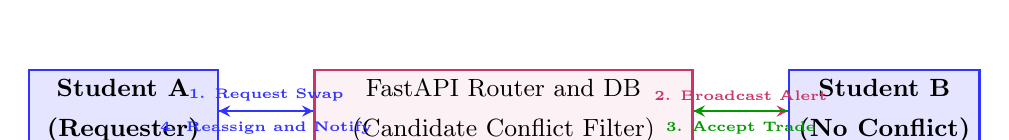
\begin{tikzpicture}[
    node distance=1.2cm,
    actor/.style={rectangle, draw=blue!80, fill=blue!10, thick, minimum width=2.4cm, minimum height=1.0cm, font=\small\bfseries, align=center},
    process/.style={rectangle, draw=purple!80, fill=purple!5, thick, minimum width=4.8cm, minimum height=1.0cm, font=\small, align=center}
]
    \node (a) [actor] {Student A\\(Requester)};
    \node (api) [process, right=of a] {FastAPI Router and DB\\(Candidate Conflict Filter)};
    \node (b) [actor, right=of api] {Student B\\(No Conflict)};

    \draw[->, >=stealth, thick, blue!80] (a) -- node[above, font=\tiny\bfseries]{1. Request Swap} (api);
    \draw[->, >=stealth, thick, purple!80] (api) -- node[above, font=\tiny\bfseries]{2. Broadcast Alert} (b);
    \draw[->, >=stealth, thick, green!60!black] (b) -- node[below, font=\tiny\bfseries]{3. Accept Trade} (api);
    \draw[->, >=stealth, thick, blue!80] (api) -- node[below, font=\tiny\bfseries]{4. Reassign and Notify} (a);
\end{tikzpicture}%
}
\caption{Shift Swap Broadcast Matching Engine Sequence Flow}
\label{fig:swap_sequence}
\end{figure}

% ================= SECTION 5 =================
\section{System API Directory}
The SoD Management System APIs are grouped into 5 modular scopes, exposing clean RESTful handlers.

\begin{table}[H]
\centering
\caption{System API Endpoint Directory}
\label{tab:api_directory}
\resizebox{0.95\linewidth}{!}{%
\begin{tabular}{lc|l|l|c}
\toprule
\textbf{Module} & \textbf{Method} & \textbf{Endpoint Path} & \textbf{Description} & \textbf{Access Scope} \\
\midrule
Auth & \texttt{POST} & \texttt{/api/v1/auth/register} & Registers new user profile & Public \\
Auth & \texttt{POST} & \texttt{/api/v1/auth/login} & Validates credentials and issues JWT & Public \\
Auth & \texttt{GET} & \texttt{/api/v1/auth/students} & Lists all registered student accounts & Registered Users \\
\midrule
Schedule & \texttt{POST} & \texttt{/api/v1/schedule/parse} & Regex parsing of copy-pasted IRAS text & Student \\
Schedule & \texttt{GET} & \texttt{/api/v1/schedule/me} & Fetches active user weekly timetable slots & Student \\
Schedule & \texttt{POST} & \texttt{/api/v1/schedule/override} & Toggles busy manual override state & Student \\
Schedule & \texttt{GET} & \texttt{/api/v1/schedule/student/\{id\}} & Fetches target student schedule slots & Supervisor / Manager \\
\midrule
Duties & \texttt{POST} & \texttt{/api/v1/tasks} & Creates duty shift slot (validates conflicts) & Manager \\
Duties & \texttt{GET} & \texttt{/api/v1/tasks} & Lists duty slots (filtered by user context) & All Roles \\
Duties & \texttt{PATCH} & \texttt{/api/v1/tasks/\{id\}} & Assigns student or edits notes / completion & All Roles (Scoped) \\
Duties & \texttt{DELETE} & \texttt{/api/v1/tasks/\{id\}} & Deletes duty slot & Manager \\
\midrule
Swaps & \texttt{POST} & \texttt{/api/v1/swaps/request} & Requests shift trade (public/private) & Student \\
Swaps & \texttt{GET} & \texttt{/api/v1/swaps} & Lists pending and accepted swap requests & All Roles (Scoped) \\
Swaps & \texttt{POST} & \texttt{/api/v1/swaps/\{id\}/respond} & Accepts or declines a trade offer & Student \\
\midrule
Billing & \texttt{POST} & \texttt{/api/v1/billing/submit} & Submits monthly hourly claim sheet & Student \\
Billing & \texttt{GET} & \texttt{/api/v1/billing/claims} & Lists claims (filtered by status / student) & All Roles (Scoped) \\
Billing & \texttt{POST} & \texttt{/api/v1/billing/\{id\}/approve} & Multi-stage approvals (verify/approve/pay) & Faculty / Manager \\
Billing & \texttt{GET} & \texttt{/api/v1/billing/export} & Downloads payroll report in CSV format & Faculty / Manager \\
\bottomrule
\end{tabular}%
}
\end{table}

% ================= SECTION 6 =================
\section{SDLC Verification (V-Model Mapping)}
Every functional requirement and user story is tied to automated integration testing files under \texttt{backend/tests/} to guarantee coverage and prevent regressions.

\begin{table}[H]
\centering
\caption{SDLC Requirements Verification Mapping}
\label{tab:vmodel}
\resizebox{0.95\linewidth}{!}{%
\begin{tabular}{lp{4cm}p{4cm}l}
\toprule
\textbf{User Story} & \textbf{Requirements Scope} & \textbf{Verification Target} & \textbf{Test File Path} \\
\midrule
US-001 / US-002 & User Registration \& JWT Login & Successful register, duplicate checks, token & \texttt{backend/tests/test\_auth.py} \\
US-004 & IRAS Schedule Parser & UTF-8 parsing, extraction of days and hours & \texttt{backend/tests/test\_schedule.py} \\
US-005 / US-006 & Availability Grid \& Overrides & Manual toggle of overrides, database saving & \texttt{backend/tests/test\_schedule.py} \\
US-007 / US-010 & Duty Slots CRUD \& Conflicts & Prevent overlapping assignment, CRUD controls & \texttt{backend/tests/test\_duty.py} \\
US-008 / US-011 & Swap Request \& Inbox & Overlap-free candidate notification routing & \texttt{backend/tests/test\_swap.py} \\
US-012 / US-013 & Billing Pipeline \& CSV Export & Double-submission guard, CSV streaming & \texttt{backend/tests/test\_billing.py} \\
\bottomrule
\end{tabular}%
}
\end{table}

\begin{table}[H]
\centering
\caption{Automated Pytest Execution Summary}
\label{tab:pytest}
\resizebox{0.95\linewidth}{!}{%
\begin{tabular}{lccc}
\toprule
\textbf{Test Module} & \textbf{Test Cases} & \textbf{Passed} & \textbf{Pass Rate} \\
\midrule
\texttt{test\_auth.py} & 5 & 5 & 100\% \\
\texttt{test\_billing.py} & 1 & 1 & 100\% \\
\texttt{test\_duty.py} & 2 & 2 & 100\% \\
\texttt{test\_schedule.py} & 7 & 7 & 100\% \\
\texttt{test\_swap.py} & 1 & 1 & 100\% \\
\textbf{Total} & \textbf{16} & \textbf{16} & \textbf{100\%} \\
\bottomrule
\end{tabular}%
}
\end{table}

% ================= SECTION 7 =================
\section{Retrospective \& Future Roadmap Backlog}

\subsection{Lessons Learned}
\begin{enumerate}
    \item \textbf{SQLite Type Mappings:} Storing time fields as ISO-formatted string boundaries (\texttt{HH:MM}) allowed async comparison operators (\texttt{<}, \texttt{>}) to execute fast in both SQLite and PostgreSQL.
    \item \textbf{Decoupled Business Hooks:} Consolidating state managers into isolated hooks (like \texttt{useSchedule.ts}) facilitated easy API migrations from mock states to FastAPI endpoints.
\end{enumerate}

\subsection{Future Roadmap Backlog}
\begin{itemize}
    \item \textbf{Live WebSockets:} Replace 10-second polling loops with active WebSocket connections to push instant notifications.
    \item \textbf{Faculty Email Triggers:} Implement SMTP email alerts when a billing claim is submitted for verification.
    \item \textbf{Mobile Adaptability:} Port visual schedule grids to responsive native mobile app grids.
\end{itemize}

% ================= REFERENCES =================
\section{References}
\begin{thebibliography}{9}

\bibitem{b1}
FastAPI Framework Documentation. "Asynchronous Web Framework for Python." (2026). \\
\url{https://fastapi.tiangolo.com/}

\bibitem{b2}
React Documentation. "A JavaScript library for building user interfaces." Meta Platforms. (2026). \\
\url{https://react.dev/}

\bibitem{b3}
SQLAlchemy ORM Documentation. "The Python SQL Toolkit and Object Relational Mapper." (2026). \\
\url{https://www.sqlalchemy.org/}

\bibitem{b4}
Pydantic Data Validation. "Data validation and settings management using Python type hints." (2026). \\
\url{https://docs.pydantic.dev/}

\bibitem{b5}
ISO/IEC 14443. "Identification cards -- Contactless integrated circuit cards -- Proximity cards." International Organization for Standardization. (2020).

\bibitem{b6}
Sommerville, Ian. "Software Engineering." 10th Edition, Pearson Education. (2016).

\end{thebibliography}

\end{document}
